\documentclass[10pt,a4paper]{article}

% ===== Fonts (xelatex) =====
\usepackage{fontspec}
\defaultfontfeatures{Ligatures=TeX}
\newcommand{\tgpath}{/usr/local/texlive/2022/texmf-dist/fonts/opentype/public/tex-gyre/}
\setmainfont[
  Path           = \tgpath,
  Extension      = .otf,
  UprightFont    = texgyrepagella-regular,
  BoldFont       = texgyrepagella-bold,
  ItalicFont     = texgyrepagella-italic,
  BoldItalicFont = texgyrepagella-bolditalic,
]{TeX Gyre Pagella}
\setsansfont[
  Path           = \tgpath,
  Extension      = .otf,
  Scale          = 0.94,
  UprightFont    = texgyreheros-regular,
  BoldFont       = texgyreheros-bold,
  ItalicFont     = texgyreheros-italic,
  BoldItalicFont = texgyreheros-bolditalic,
]{TeX Gyre Heros}
\setmonofont[
  Path           = \tgpath,
  Extension      = .otf,
  Scale          = 0.86,
  UprightFont    = texgyrecursor-regular,
  BoldFont       = texgyrecursor-bold,
  ItalicFont     = texgyrecursor-italic,
  BoldItalicFont = texgyrecursor-bolditalic,
]{TeX Gyre Cursor}

% ===== Page layout =====
\usepackage[a4paper, top=1.7cm, bottom=1.8cm, left=2.0cm, right=2.0cm]{geometry}
\usepackage{microtype}

% ===== Color palette =====
\usepackage[dvipsnames,table]{xcolor}
\definecolor{primary}{HTML}{1F3A5F}
\definecolor{accent}{HTML}{0E7C86}
\definecolor{softgray}{HTML}{F4F5F7}
\definecolor{rulegray}{HTML}{C5CAD1}
\definecolor{mutedtext}{HTML}{4A5568}
\definecolor{warm}{HTML}{C2410C}
\definecolor{success}{HTML}{059669}
\definecolor{fail}{HTML}{B91C1C}
\definecolor{rowalt}{HTML}{FAFBFC}

% ===== Core packages =====
\usepackage{url}
\usepackage{amsmath,amssymb}
\usepackage{graphicx}
\usepackage{float}
\usepackage{needspace}
\usepackage{subcaption}
\usepackage{booktabs}
\usepackage{tikz}
\usepackage{enumitem}
\usepackage{titling}
\usepackage{titlesec}
\usepackage{authblk}
\usepackage{caption}
\usepackage[most]{tcolorbox}
\usepackage{fancyhdr}
\usepackage{lastpage}
\usepackage{multicol}
\usepackage{listings}
\usepackage{hyperref}
\usetikzlibrary{arrows.meta, positioning, shapes.geometric, fit, backgrounds, calc, shadows.blur}

% ===== Spacing & lists =====
\linespread{1.04}
\setlength{\parskip}{2pt}
\setlength{\parindent}{0pt}
\setlength{\floatsep}{5pt plus 1pt minus 1pt}
\setlength{\textfloatsep}{6pt plus 1pt minus 2pt}
\setlength{\intextsep}{5pt plus 1pt minus 1pt}
\renewcommand{\arraystretch}{1.05}
\renewcommand{\figurename}{Fig.}
\renewcommand{\tablename}{Tab.}

\setlist[itemize]{leftmargin=1.3em, itemsep=1.6pt, parsep=0pt, topsep=2pt,
                  label={\color{accent}\footnotesize$\blacktriangleright$}}
\setlist[enumerate]{leftmargin=1.6em, itemsep=1.6pt, parsep=0pt, topsep=2pt,
                    label={\color{primary}\sffamily\bfseries\arabic*.}}

% ===== Section headings =====
\titleformat{\section}[hang]
  {\sffamily\large\bfseries\color{primary}}
  {\colorbox{primary}{\color{white}\sffamily\bfseries\,\thesection\,}\hspace{0.6em}}
  {0pt}{}
  [\vspace{1pt}{\color{rulegray}\rule{\linewidth}{0.4pt}}]
\titleformat{\subsection}[hang]
  {\sffamily\normalsize\bfseries\color{accent}}
  {\thesubsection}{0.5em}{}
\titleformat{\subsubsection}[runin]
  {\sffamily\normalsize\bfseries\color{primary}}
  {}{0pt}{}[~---~]
\titlespacing{\section}{0pt}{9pt plus 2pt minus 1pt}{4pt}
\titlespacing{\subsection}{0pt}{6pt}{2pt}
\titlespacing{\subsubsection}{0pt}{4pt}{0pt}

% ===== Caption styling =====
\captionsetup{font=small, labelfont={sf,bf,color=primary}, labelsep=period,
              skip=3pt, justification=justified}
\captionsetup[sub]{font=footnotesize, labelfont={sf,bf,color=accent}, labelsep=period, skip=2pt}

% ===== Boxed elements =====
\newtcolorbox{infobox}{
  enhanced, colback=softgray, colframe=rulegray, boxrule=0.3pt,
  arc=2pt, left=8pt, right=8pt, top=5pt, bottom=5pt,
  before skip=2pt, after skip=4pt,
  borderline west={2.2pt}{0pt}{accent},
}
\newtcolorbox{successbox}{
  enhanced, colback=success!4, colframe=success!40, boxrule=0.3pt,
  arc=2pt, left=8pt, right=8pt, top=4pt, bottom=4pt,
  before skip=2pt, after skip=4pt,
  borderline west={2.2pt}{0pt}{success},
}
\newtcolorbox{failbox}{
  enhanced, colback=fail!4, colframe=fail!40, boxrule=0.3pt,
  arc=2pt, left=8pt, right=8pt, top=4pt, bottom=4pt,
  before skip=2pt, after skip=4pt,
  borderline west={2.2pt}{0pt}{fail},
}
\newtcolorbox{insightbox}{
  enhanced, colback=accent!4, colframe=accent!35, boxrule=0.3pt,
  arc=2pt, left=8pt, right=8pt, top=4pt, bottom=4pt,
  before skip=3pt, after skip=4pt,
  borderline west={2.2pt}{0pt}{accent},
}

% ===== Code listings =====
\lstdefinestyle{tinypy}{
  basicstyle=\ttfamily\scriptsize,
  language=Python,
  keywordstyle=\color{primary}\bfseries,
  commentstyle=\color{success}\itshape,
  stringstyle=\color{warm},
  numbers=none,
  showstringspaces=false,
  breaklines=true,
  frame=none,
  xleftmargin=10pt,
  aboveskip=2pt,
  belowskip=2pt,
}

% ===== URLs / hyperlinks =====
\hypersetup{colorlinks=true, urlcolor=accent, linkcolor=primary, citecolor=primary,
            breaklinks=true}
\sloppy
\emergencystretch=1.5em

% ===== Page footer =====
\pagestyle{fancy}
\fancyhf{}
\renewcommand{\headrulewidth}{0pt}
\renewcommand{\footrulewidth}{0pt}
\fancyfoot[L]{\scriptsize\sffamily\color{mutedtext}Context-Aware Emotional TTS\,\textbullet\,MAIE5531 Final Report}
\fancyfoot[R]{\scriptsize\sffamily\color{mutedtext}\thepage\ / \pageref*{LastPage}}

% ===== Title block =====
% Visual hierarchy:
%   Title  +-- 1pt  --+ Subtitle                (one semantic group: tight)
%                                               <--- ~1em gap --->
%   Authors          +-- 1pt --+ Affiliation    (one semantic group: tight)
%                                               <--- ~1em gap --->
%   Abstract
\setlength{\droptitle}{-1.2em}
\pretitle{\begin{center}\sffamily\bfseries\Large\color{primary}}
\posttitle{\par\end{center}\vspace{0.4em}}
\preauthor{\begin{center}\sffamily\small\color{mutedtext}}
\postauthor{\end{center}\vspace{-1.2em}}
\predate{}\postdate{}\date{}
\renewcommand\Affilfont{\sffamily\scriptsize\itshape\color{mutedtext}}
\setlength{\affilsep}{2pt}   % keep authors & affiliation visually glued
\setcounter{secnumdepth}{3}

\title{Context-Aware Emotional TTS for Game AI Dubbing\\[1pt]
  {\normalsize\sffamily\mdseries\itshape\color{mutedtext}%
   Final Report\,\textbullet\,MAIE5531 GenAI and LLM\,\textbullet\,May 2026}}
\author[1]{HE Yunlin}
\author[1]{WANG Yifu}
\author[1]{SU Ziyao}
\author[1]{HAN Shipeng}
\affil[1]{AI \& Entrepreneurship, Hong Kong University of Science and Technology}

\begin{document}
\maketitle
\thispagestyle{fancy}

\vspace{0.4em}
\begin{infobox}
\noindent\small
{\sffamily\bfseries\color{primary}Abstract.}~%
Narrative-driven games depend on tens of thousands of voiced lines, but most
neural voice cloners only solve the \emph{timbre} side and leave the
\emph{performance} flat across scenes. We build an end-to-end emotional dubbing
pipeline on top of \textbf{28~min} of in-character data: a Qwen3-TTS\,1.7B
\textbf{voice cloner} (full SFT, v5\,ep3, SIM\textsubscript{gt}\,=\,\textbf{0.689},
WER\,=\,\textbf{4.25\,\%}, RTF\,=\,\textbf{0.357} via FasterQwen3TTS CUDA Graph),
fronted by an \textbf{LLM-as-emotional-director} that emits a strict
\texttt{EmotionAnnotation} JSON (emotion, intensity, pace, style, reference
emotion category, Fish-style inline tags), grounded by a \textbf{Character RAG}
and a \textbf{10-turn Emotion Arc Tracker}, and dispatched through an
\textbf{eight-backend TTS router} that includes a SIM-cosine quality gate
trading emotion expressiveness against timbre drift. The full pipeline is
served via FastAPI and visualised in a React app with an offline Demo Mode.
On A100 we measure end-to-end latency of $\sim$10.5\,s/sentence (LLM
67\,\%, RAG 13\,\%, TTS 19\,\%), independently re-verify the 3.9$\times$
CUDA-Graph speed-up, and report SIM\textsubscript{ref}/WER for three pipeline
conditions. We also document a $+141\,\%$ SIM bug fix in bf16 speaker-embedding
accumulation, and three architecturally infeasible acceleration attempts
(INT8, speculative decoding, self-speculative early-exit) whose failure modes
inform the future-work direction.\\[2pt]
{\sffamily\bfseries\color{primary}Keywords.}~Emotional TTS~\textbullet~Voice Cloning~\textbullet~Retrieval-Augmented Generation~\textbullet~LLM~\textbullet~Game AI Dubbing~\textbullet~CUDA Graph Inference
\end{infobox}

\vspace{1pt}

%% ============================================================
\section{Introduction}
%% ============================================================

Voice acting is one of the largest line-items in modern game production:
industry estimates put it at \textbf{10--15\,\%} of a AAA budget, and
narrative-driven titles such as otome / dating sims can carry tens of
thousands of voiced lines per character. Iterating on script edits, adding
DLC, or localising to a new language each requires re-recording sessions on
a tight studio calendar.

Recent open-source TTS models -- Qwen3-TTS, Fish Speech, CosyVoice, GPT-SoVITS
-- close the timbre gap with as little as 30\,minutes of target-speaker audio.
But once we ship those clones into an actual scene, a second problem
surfaces: \emph{the cloned voice sounds the same in every line}. A character
who is comforting the player after a near-miss should not deliver the line
with the same neutral cadence as a tutorial system message; a villain
threatening the protagonist should not sound clinically polite. The
performance side -- pace, timbral colour, micro-prosody, scene-grounded
emotion -- is what a human voice director normally provides, and what AI
cloners do not.

\paragraph{Our thesis.} \emph{The audible gap between cloned timbre and
cloned performance can be closed by engineering a pipeline, rather than by
training a much larger model.} We replace the human director with three
software layers stacked in front of a Qwen3-TTS clone:

\begin{enumerate}
  \item An \textbf{LLM Context Engine} (GPT-4o) that reads the scene
        description plus the dialogue and produces a strict, validated
        \texttt{EmotionAnnotation} schema -- not free-form prompt text,
        but a Pydantic-typed contract that downstream backends can act on
        deterministically.
  \item A \textbf{Character Knowledge RAG} (bge-large-zh-v1.5 + ChromaDB
        over four hand-curated markdown files) that injects in-character
        habits and constraints into the LLM prompt.
  \item An \textbf{Emotion Arc Tracker} that maintains a 10-turn sliding
        window of past states so the LLM can avoid abrupt jumps and
        reproduce believable emotional progression.
\end{enumerate}

These feed an \textbf{eight-backend TTS dispatcher} that picks per-emotion
reference audio, blends emotion-conditioned and timbre-only synthesis under
a speaker-similarity quality gate, and exposes a single FastAPI endpoint
that powers a React front end with an offline Demo Mode for unblocked UX
iteration on a single shared GPU.

The paper is organised around the project's chronological story. \S2 covers
\textbf{Phase~1 -- Voice Cloning Foundation} (data pipeline, five fine-tuning
iterations, the bf16 speaker-embedding bug, inference acceleration). \S3
covers \textbf{Phase~2 -- the Emotional Context Pipeline} (the three new
layers and the dispatcher). \S4 reports our \textbf{end-to-end evaluation on
A100}. \S5 honestly enumerates the \textbf{three architecturally-infeasible
acceleration attempts}, the LR/data missteps, and the upstream training
bugs we may also have inherited. \S6 distils the \textbf{five remaining
bottlenecks}, and \S7 maps each one to a \textbf{web-research-backed
solution} ranked by ROI.

%% ============================================================
\section{Phase 1 --- Voice Cloning Foundation}
%% ============================================================

\subsection{Data pipeline (664 clips, $\sim$28~min)}

Our target speaker is the male character ``Qinche'' (秦彻) from the Chinese
otome game \emph{Lovebrush Chronicles}. Source material is publicly available
fan-edited Bilibili videos (single-speaker game cutscenes); only audio
without copyrighted background music is used. Fig.~\ref{fig:pipeline}
summarises the pipeline:

\begin{enumerate}
  \item \textbf{Demucs} for vocals separation when the source has BGM;
  \item \textbf{pyannote diarization} on the (rare) mixed-source clips to
        keep only Qinche's segments;
  \item \textbf{silero-VAD} to cut into 1--15\,s utterances;
  \item \textbf{WhisperX large-v3} for Mandarin transcription;
  \item \textbf{OpenCC} traditional$\to$simplified normalisation;
  \item a \textbf{purification pass} (\texttt{purify\_dataset.py})
        that runs a speaker-similarity filter and produces a 90:10
        train/test split;
  \item \textbf{RMS normalisation + 1\,s tail-silence pad}
        (\texttt{normalize\_audio.py}) so reference and generated
        clips occupy the same loudness/silence regime.
\end{enumerate}

The final v5 corpus contains \textbf{664} clips totalling
$\sim$28~minutes (mean clip length 2.5\,s; cf.~Fig.~\ref{fig:datadist}).
A frozen 18-clip evaluation set is held out, plus 5 reference clips for
zero-shot prompting and a hand-curated \textbf{6-bucket emotion library}
(5 clips each) used by the Phase-2 dispatcher.

\begin{figure}[t]
\centering
\begin{subfigure}[t]{0.49\linewidth}
  \centering
  \includegraphics[width=\linewidth]{figs/preprocessing_pipeline.pdf}
  \caption{Audio preprocessing pipeline.}
  \label{fig:pipeline}
\end{subfigure}\hfill
\begin{subfigure}[t]{0.49\linewidth}
  \centering
  \includegraphics[width=\linewidth]{figs/dataset_duration_distribution.pdf}
  \caption{Clip duration distribution (v5, 664 clips, $\sim$28\,min).}
  \label{fig:datadist}
\end{subfigure}
\caption{\textbf{Data pipeline and dataset statistics.} Bilibili audio is
processed end-to-end into 1--15\,s utterances; the v5 distribution is
right-skewed with a mean of 2.5\,s.}
\label{fig:data}
\end{figure}

\subsection{Five fine-tuning iterations}

We train Qwen3-TTS-12Hz-1.7B-Base (Apache-2.0) with full SFT on 8$\times$A100
SXM4-80GB, PyTorch 2.6, FlashAttention~2. Five revisions evolved both
hyper-parameters and the dataset; Tab.~\ref{tab:p1iters} summarises the
trajectory. Three observations matter for the rest of the report:

\begin{itemize}
  \item \textbf{LR sensitivity is ferocious.} v3 used 1e-5 (the official
        default), which converged faster on the training loss but degraded
        SIM\textsubscript{gt}; we settled on 2e-6 for v2/v4/v5. The
        community LoRA recipe~\cite{instavar2026} independently reports
        the same direction.
  \item \textbf{Data quality $>$ data quantity.} v6 added 74 \texttt{nobgm}
        clips (+16\,\% data) but SIM\textsubscript{gt} \emph{dropped} by
        $\sim$0.01; the BGM-removal residue confused the speaker encoder.
        We reverted.
  \item \textbf{The bf16 speaker-embedding accumulation bug masked our true
        ceiling for two months.} See \S2.3.
\end{itemize}

\begin{table}[t]
\centering\small
\caption{\textbf{Five fine-tuning iterations.} Best-epoch numbers reported
on the 18-clip held-out test set; SIM\textsubscript{gt} is cosine
similarity against ground-truth reference embeddings; RTF measured with
FasterQwen3TTS where applicable. v5 ep3 is our shipped model.}
\label{tab:p1iters}
\rowcolors{2}{rowalt}{white}
\footnotesize
\begin{tabular}{@{}llccccl@{}}
\toprule
\textbf{Ver} & \textbf{LR / sched.} & \textbf{Data} &
\textbf{SIM\textsubscript{gt}} & \textbf{WER} & \textbf{RTF} &
\textbf{Verdict} \\
\midrule
v1               & 2e-5, none           & 387             & 0.04--0.10 & 2.9--4.4     & --             & failed (no sched., spk-emb bug) \\
v2 (buggy)       & 2e-6, warm10\%+cos.  & 461             & 0.21--0.29 & 0.02--0.03   & 2.58           & bf16 spk-emb bug undetected \\
v2 (fixed)       & 2e-6                 & 461             & \textbf{0.696} & 0.0365   & 2.58           & post-hoc fp32 fix \\
v3               & \textbf{1e-5}        & 461             & 0.66--0.68 & 0.029--0.038 & 2.43           & higher LR $\ne$ better \\
v4               & 2e-6                 & 461             & 0.678      & 0.053        & \textbf{0.351} & FastQwen integrated \\
\rowcolor{success!8}
\textbf{v5}      & 2e-6                 & \textbf{664}    & \textbf{0.6892} & \textbf{0.0425} & \textbf{0.357} & shipped \\
v6               & 2e-6                 & 738 (+74 noisy) & 0.68       & ---          & 0.36           & reverted \\
\bottomrule
\end{tabular}
\end{table}

\subsection{The bf16 speaker-embedding bug -- our biggest single lever}

Qwen3-TTS conditions speech on a learnt speaker embedding; the trainer
accumulates per-clip embeddings produced by the speaker encoder and writes
out the running mean. The default code keeps both the per-clip output and
the accumulator in \texttt{bfloat16}:

\begin{lstlisting}[style=tinypy]
spk_embed_sum += spk_encoder(wav)             # buggy: bf16 accumulation
spk_embed = spk_embed_sum / N                 # norm collapses to ~2.98
\end{lstlisting}

After a few hundred batches the running sum's norm \emph{collapses} from the
$\sim$17 of a single embedding to $\sim$2.98 because the bf16 mantissa cannot
represent the small per-step delta. The trained checkpoint then ``points''
nowhere near the real speaker. The fix is one line:

\begin{lstlisting}[style=tinypy]
spk_embed_sum += spk_encoder(wav).float()     # accumulate in fp32
spk_embed = (spk_embed_sum / N).bfloat16()    # cast back at save
\end{lstlisting}

The lift was $+141\,\%$ on SIM\textsubscript{gt} ($\sim$0.29 $\to$
$\sim$0.70; Fig.~\ref{fig:bf16}). This is the single biggest quality
intervention in the entire project.

\begin{insightbox}\small
\textbf{Lesson.} Any \emph{accumulate-then-normalise} metric trained under
\texttt{mixed\_precision="bf16"} needs an fp32 detour. Standard
mixed-precision tutorials never warn about this because token-loss
accumulation is not norm-sensitive -- but speaker-embedding cosine is.
\end{insightbox}

\subsection{Inference acceleration}

We tried five ideas (Tab.~\ref{tab:accel}); only \textbf{CUDA Graph} (the
internal trick used by \texttt{FasterQwen3TTS}) survived. The three failed
attempts give us a clean view of what kinds of LLM tricks port to TTS and
which do not -- discussed honestly in \S5.

\begin{table}[t]
\centering\small
\caption{\textbf{Inference acceleration attempts (Phase 1).} Only CUDA
Graph survived; the three failed methods inform our future-work direction.
Numbers measured on 18-clip held-out set with FasterQwen3TTS where
applicable.}
\label{tab:accel}
\rowcolors{2}{rowalt}{white}
\footnotesize
\begin{tabular}{@{}lccll@{}}
\toprule
\textbf{Method} & \textbf{RTF (orig)} & \textbf{RTF (opt)} &
\textbf{Quality} & \textbf{Status} \\
\midrule
\rowcolor{success!8}
\textbf{FasterQwen3TTS (CUDA Graph)} & 2.542 & \textbf{0.357} & lossless     & shipped, $\times7.1$ \\
Fish Speech \texttt{--compile}        & 4.315 & 0.639          & lossless     & verified \\
Flash-Attention 2                     & ---    & ---            & lossless     & default-on \\
\rowcolor{fail!7}
INT8 (bitsandbytes)                   & 0.357  & $\approx$7.0   & broken (SIM 0.07 / WER 1.0) & \textbf{failed} \\
\rowcolor{fail!7}
Speculative dec.\ (0.6B Base draft)    & ---    & slower         & accept rate 0--5\,\% & \textbf{failed} \\
\rowcolor{fail!7}
Self-speculative / early-exit         & ---    & ---            & mid-layer agreement $<$\,7\,\% & \textbf{failed} \\
\bottomrule
\end{tabular}
\end{table}

\subsection{Phase-1 final numbers}

Tab.~\ref{tab:p1final} consolidates the head-to-head against the
zero-shot Qwen3-TTS baseline and the Fish~Audio S2~Pro reference TTS.
Two key takeaways:
(i)~v5\,ep3 \emph{matches} Qwen ZS on SIM\textsubscript{gt} while
\textbf{cutting WER by $\sim$3$\times$} (4.25\,\% vs.\ 12.03\,\%);
(ii)~v5\,ep3 \emph{dominates} Fish~S2~Pro on SIM\textsubscript{gt}
(0.689 vs.\ 0.663) at comparable RTF after compilation.
Fig.~\ref{fig:phase1nums} visualises the comparison alongside the curated
6-bucket emotion library used by Phase~2.

\begin{table}[t]
\centering\small
\caption{\textbf{Phase-1 final numbers.} 18-clip held-out test set, full
audio. CUDA-Graph inference gives a 7$\times$ RTF reduction at no quality
cost. The \textbf{v5 ep3} row is our shipped configuration.}
\label{tab:p1final}
\rowcolors{2}{rowalt}{white}
\footnotesize
\begin{tabular}{@{}lcccccl@{}}
\toprule
\textbf{Model / setting} & \textbf{SIM\textsubscript{gt}} &
\textbf{SIM\textsubscript{ref}} & \textbf{WER} & \textbf{RTF} &
\textbf{Inference} \\
\midrule
Qwen3 1.7B Zero-shot                         & \textbf{0.7104} & 0.7563 & 0.1203 & 2.401 & native \\
\rowcolor{success!8}
\textbf{Qwen3 SFT v5 ep3 (ours)}             & \textbf{0.6892} & 0.7161 & 0.0425 & \textbf{0.357} & FasterQwen3TTS \\
Qwen3 SFT v5 ep3 (native baseline)           & 0.6885 & \textbf{0.7281} & 0.0451 & 2.542 & native \\
Qwen3 SFT v5 ep5                             & 0.6791 & 0.6998 & \textbf{0.0279} & 0.356 & FasterQwen3TTS \\
Qwen3 SFT v5 ep9                             & 0.6795 & 0.7180 & \textbf{0.0269} & 0.354 & FasterQwen3TTS \\
Fish~S2~Pro Zero-shot (\texttt{--compile})    & 0.6627 & 0.6824 & 0.0209 & 0.639 & torch.compile \\
\bottomrule
\end{tabular}
\end{table}

\begin{figure}[t]
\centering
\begin{subfigure}[t]{0.495\linewidth}
  \centering
  \includegraphics[width=\linewidth]{figs/bf16_bug_impact.pdf}
  \caption{The bf16 spk-emb accumulation bug: SIM\textsubscript{gt} jumps from $\sim$0.29 to $\sim$0.70 after the fp32-accumulation fix ($+141\,\%$).}
  \label{fig:bf16}
\end{subfigure}\hfill
\begin{subfigure}[t]{0.495\linewidth}
  \centering
  \includegraphics[width=\linewidth]{figs/rtf_comparison_bar.pdf}
  \caption{Inference acceleration: FasterQwen3TTS CUDA Graph drops RTF from 2.54 to 0.357 ($7.1\times$); INT8 / speculative decoding / early-exit all failed (\S5).}
  \label{fig:rtf}
\end{subfigure}
\caption{\textbf{The two largest Phase-1 wins:} a one-line bf16 fix and a CUDA-Graph integration. Together they took the project from ``not converging'' to ``real-time, near zero-shot quality, lower WER.''}
\label{fig:phase1milestones}
\end{figure}

\begin{figure}[t]
\centering
\includegraphics[width=0.92\linewidth]{figs/emotion_and_phase1.pdf}
\caption{\textbf{(a)} The 6-bucket emotion library (5 curated reference clips per category, used by the Phase-2 dispatcher). \textbf{(b)} Phase-1 head-to-head: v5\,ep3 matches Qwen ZS on SIM and beats Fish~S2~Pro on SIM at similar WER.}
\label{fig:phase1nums}
\end{figure}

%% ============================================================
\section{Phase 2 --- Emotional-Aware Context Pipeline}
%% ============================================================

Phase~1 left us with a real-time, in-character voice. Phase~2 builds the
\emph{director}: a software stack that, given only a scene description and
the next dialogue line, decides \emph{how} the line should be performed,
selects matching reference audio, dispatches to the right TTS backend, and
preserves continuity across turns. Fig.~\ref{fig:arch} is the full picture.

\begin{figure}[t]
\centering
\definecolor{cIn}{HTML}{4F83CC}
\definecolor{cRag}{HTML}{0E7C86}
\definecolor{cLlm}{HTML}{7C3AED}
\definecolor{cArc}{HTML}{D97706}
\definecolor{cTts}{HTML}{059669}
\definecolor{cOut}{HTML}{334155}
\definecolor{cApi}{HTML}{C2410C}
\resizebox{\linewidth}{!}{%
\begin{tikzpicture}[
  font=\sffamily\scriptsize,
  >=Latex,
  block/.style={rectangle, rounded corners=3pt, draw=black!30, line width=0.4pt,
                minimum height=9mm, inner xsep=5pt, inner ysep=3pt,
                align=center, fill=white,
                blur shadow={shadow blur steps=4, shadow opacity=15,
                             shadow xshift=0.5pt, shadow yshift=-0.6pt}},
  inp/.style={block, top color=cIn!14,  bottom color=cIn!3,  draw=cIn!55},
  rg/.style={block,  top color=cRag!16, bottom color=cRag!3, draw=cRag!55},
  ll/.style={block,  top color=cLlm!16, bottom color=cLlm!3, draw=cLlm!55},
  ac/.style={block,  top color=cArc!22, bottom color=cArc!4, draw=cArc!60},
  tt/.style={block,  top color=cTts!16, bottom color=cTts!3, draw=cTts!55},
  ttplus/.style={block, top color=cTts!26, bottom color=cTts!7, draw=cTts!65},
  op/.style={block,  top color=cOut!12, bottom color=cOut!3, draw=cOut!50},
  ap/.style={block,  top color=cApi!14, bottom color=cApi!3, draw=cApi!55,
             minimum height=7mm},
  lbl/.style={font=\sffamily\scriptsize\bfseries},
  arr/.style={->, draw=black!55, line width=0.55pt,
              shorten >=1.5pt, shorten <=1.5pt},
  fb/.style ={->, draw=cArc!70, line width=0.5pt, dashed,
              shorten >=1.5pt, shorten <=1.5pt},
  loop/.style={->, draw=black!30, line width=0.45pt, dashed,
               shorten >=1.5pt, shorten <=1.5pt},
  group/.style={rectangle, rounded corners=4pt, draw=#1!50, dashed,
                line width=0.4pt, fill=#1!4, inner sep=4pt}
]

% ============================================================
% ROW 1 — Scene  →  RAG (KB+Chroma)  →  LLM ⇆ Arc  →  Annotation
% ============================================================
\node[inp, minimum width=22mm]                  (scene)  {Scene description \\ + dialogue list};
\node[rg,  right=10mm of scene, minimum width=20mm] (kb)     {Character KB \\ \tiny(4 md files)};
\node[rg,  right=4mm  of kb,    minimum width=20mm] (chroma) {ChromaDB \\ \tiny(bge-large-zh-v1.5)};
\node[ll,  right=10mm of chroma, minimum width=24mm] (llm)   {LLM Emotion Analyzer \\ \tiny(GPT-4o via OpenRouter)};
\node[op,  right=10mm of llm,   minimum width=30mm] (ann)    {\texttt{EmotionAnnotation} \\
                                                              \tiny\{emotion, intensity, pace, style, ref\_cat, fish\_tags\}};

% Arc tracker — placed under LLM, dashed feedback to LLM
\node[ac,  below=6mm of llm, minimum width=24mm] (arc) {Emotion Arc Tracker \\ \tiny(10-turn sliding window)};

% ============================================================
% ROW 2 — Ref picker → Dispatcher → {Qwen3-TTS v5, Fish S2 Pro} → .wav
% ============================================================
\node[tt,  below=20mm of kb,    minimum width=22mm] (refsel) {Ref-audio picker \\ \tiny(6 buckets $\times$ 5 clips)};
\node[tt,  right=10mm of refsel, minimum width=22mm] (disp)   {TTS Dispatcher \\ \tiny(8 backends, auto\_quality gate)};
\node[ttplus, right=14mm of disp, yshift=5mm,  minimum width=24mm] (qwen) {Qwen3-TTS v5 \\ \tiny+ FasterQwen3TTS};
\node[ttplus, right=14mm of disp, yshift=-5mm, minimum width=24mm] (fish) {Fish S2 Pro \\ \tiny(inline {[}tags{]})};
\node[op,  right=14mm of qwen, yshift=-5mm, minimum width=14mm] (wav) {\textbf{.wav}\\[-1pt]\tiny per line};

% ============================================================
% ROW 3 — Service Layer (full-width banner)
% ============================================================
\node[ap, minimum width=152mm,
      below=14mm of disp, xshift=22mm] (apisvc)
      {FastAPI server \texttt{/api/*} \quad $\longleftrightarrow$ \quad
       React visualization \,(\texttt{EmotionalTTSPage.tsx},
       Demo Mode)};

% ============================================================
% Forward arrows
% ============================================================
\draw[arr] (scene)  -- (kb);
\draw[arr] (kb)     -- (chroma);
\draw[arr] (chroma) -- (llm);
\draw[arr] (llm)    -- (ann);

% Arc tracker ↔ LLM (dashed feedback in warm orange)
\draw[fb]  (arc.north) -- node[right=0.5mm, font=\tiny\itshape, text=cArc!85]
           {feedback} (llm.south);

% Annotation drops down into the dispatcher
% Take the bend on the LEFT side of (ann) so we don't cross the (5) tts label.
\draw[arr] (ann.south west) ++(3mm,0) |- ($(disp.north)+(0,5mm)$) -- (disp.north);

% Row 2: ref + annotation feed dispatcher; dispatcher fans out
\draw[arr] (refsel) -- (disp);
\draw[arr] (disp.east) -- (qwen.west);
\draw[arr] (disp.east) -- (fish.west);
\draw[arr] (qwen.east) -- (wav.north west);
\draw[arr] (fish.east) -- (wav.south west);

% Service-layer dashed loop (audio out → API; React → new scene)
\draw[loop] (wav.south)    |- (apisvc.east);
\draw[loop] (apisvc.west) -| (scene.south);

% ============================================================
% Numbered group labels (above each section)
% ============================================================
\begin{scope}[on background layer]
\node[lbl, above=1mm of scene,                 text=cIn]   {\textsc{(1) input}};
\node[lbl, above=1mm of kb,    xshift=11mm,    text=cRag]  {\textsc{(2) character rag}};
\node[lbl, above=1mm of llm,                   text=cLlm]  {\textsc{(3) llm + arc tracker}};
\node[lbl, above=1mm of ann,                   text=cOut]  {\textsc{(4) structured output}};
\node[lbl, above=1mm of disp,                  text=cTts]  {\textsc{(5) tts}};
\node[lbl, above=1mm of apisvc, yshift=-0.2mm, text=cApi]  {\textsc{(6) service layer}};
\end{scope}

\end{tikzpicture}%
}
\caption{\textbf{End-to-end system architecture.} Three layers are new in
Phase~2: \textsc{(2)}~Character~RAG injects persona knowledge,
\textsc{(3)}~LLM~+~Emotion~Arc~Tracker turns scene + history into a strict
JSON emotion annotation, and \textsc{(5)}~the emotion-aware TTS dispatcher
routes to one of eight backends with a matching reference clip. Layers
\textsc{(1)}, \textsc{(4)} and the Phase-1 Qwen3-TTS\,v5 model were already
in place.}
\label{fig:arch}
\end{figure}

\subsection{LLM Context Engine -- structured emotion as a hard contract}

The LLM's job is intentionally narrow: read \emph{(scene description,
character KB snippet, last 10 emotion states, current line)} and emit one
\texttt{EmotionAnnotation} object. The schema (\texttt{src/context\_engine/}
\texttt{models.py}) is enforced by Pydantic v2:

\begin{lstlisting}[style=tinypy]
class EmotionAnnotation(BaseModel):
    emotion: str                        # free-form label, e.g. gentle_reassuring
    intensity: float = Field(ge=0, le=1)
    pace: Literal["slow", "normal", "fast"]
    style: str                          # natural-language stage direction
    ref_emotion_category: Literal[      # one of 6 bucketed reference categories
        "tender", "calm", "playful",
        "intense", "cold", "intimate"]
    fish_audio_tags: str                # inline [tag] annotations for Fish S2 Pro
\end{lstlisting}

We use GPT-4o via OpenRouter, \texttt{response\_format=json\_object},
temperature\,=\,0.3, with four hand-written few-shot exemplars and a 3-retry
parser. \textbf{Why a typed contract.} Free-form emotion prompts are noisy
to consume downstream (the dispatcher needs deterministic categorical
inputs to pick reference audio); strict JSON is what makes the rest of the
pipeline a pure function of the LLM output. The
\texttt{ref\_emotion\_category} is the LLM's commitment about \emph{which}
of our 6 curated reference clips should drive the cloning.

\subsection{Character RAG and the 10-turn Emotion Arc Tracker}

\textbf{Character RAG.} Four hand-curated markdown files
(\texttt{data/character\_kb/}) describe persona traits, speech idiosyncrasies,
relationships, and forbidden phrases. They are embedded with
\texttt{bge-large-zh-v1.5} into a local ChromaDB collection; each scene
retrieves the top-$k$\,=\,3 chunks and prepends them to the LLM system
prompt. We deliberately keep the KB small so that, in the future, the entire
KB can be \emph{inlined} into the prompt and runtime ChromaDB removed for
latency (see \S7.1).

\textbf{Emotion Arc Tracker.} The tracker
(\texttt{src/emotion\_tracker/tracker.py}) maintains a sliding window of the
previous 10 \texttt{EmotionAnnotation} states and a hand-tuned transition-
distance table (e.g.\ \texttt{intense}$\to$\texttt{playful} is flagged as
abrupt). Past states are fed back into the LLM system prompt, so the LLM is
nudged to produce a coherent arc rather than independently sampled per-turn
emotions.

\subsection{Eight-backend TTS dispatcher and the \texttt{auto\_quality} gate}

The dispatcher (\texttt{src/tts/}) exposes eight backends so we can A/B them
under identical prompts; Tab.~\ref{tab:backends} summarises. The two most
interesting are:

\textbf{\texttt{clone\_blend}.} Linearly interpolates between a calm-bucket
x-vector and the LLM-picked emotion-bucket x-vector, weighted by the LLM
\texttt{intensity}. This trades emotion expressiveness against timbre drift
on a continuous knob.

\textbf{\texttt{auto\_quality}.} Routes through an emotion-conditioned
backend, then computes a speaker-similarity \emph{gate}: cosine of the
generated audio's x-vector against a canonical reference. If the gate fails
(cosine $<$ 0.6, default) the dispatcher falls back to \texttt{baseline}
(timbre-only). This is the \textbf{cleanest engineering compromise} we found
between ``more emotion = more timbre drift'' -- not a clever loss
modification, just a numerical safeguard at inference.

\begin{table}[t]
\centering\small
\caption{\textbf{Eight TTS backends exposed by the dispatcher.} The
\texttt{auto\_quality} backend is the dispatcher's quality-insurance gate;
\texttt{fish} is the cross-architecture A/B baseline.}
\label{tab:backends}
\rowcolors{2}{rowalt}{white}
\footnotesize
\begin{tabular}{@{}p{0.18\linewidth}p{0.50\linewidth}p{0.26\linewidth}@{}}
\toprule
\textbf{Backend} & \textbf{Mechanism} & \textbf{Use-case} \\
\midrule
\texttt{baseline}     & SFT CustomVoice direct, no emotion injection                             & timbre upper-bound \\
\texttt{qwen}         & Qwen3-TTS zero-shot                                                      & reference baseline \\
\texttt{clone}        & SFT + single static reference clip                                       & naive cloning \\
\texttt{clone\_xvec}  & SFT + per-emotion averaged x-vector picked by LLM \texttt{ref\_cat}      & emotion-conditioned \\
\texttt{clone\_blend} & Calm $\leftrightarrow$ emotion x-vector linear interpolation by LLM intensity & continuous trade-off \\
\texttt{auto}         & Rule-based router on top of LLM output (recommended default)             & shipped UI default \\
\rowcolor{success!7}
\texttt{auto\_quality} & \texttt{auto} + SIM-cosine gate against canonical x-vector; fallback to \texttt{baseline} on gate fail & quality insurance \\
\texttt{fish}         & Fish~S2~Pro + LLM-generated inline \texttt{[tag]} annotations            & cross-arch A/B \\
\bottomrule
\end{tabular}
\end{table}

\subsection{FastAPI service and the React Demo Mode}

The full pipeline runs behind a single FastAPI server
(\texttt{src/api/server.py}) exposing four routes:
\texttt{/api/analyze} (LLM-only),
\texttt{/api/pipeline} (end-to-end),
\texttt{/api/audio/<sess>/<backend>/<file>} (audio streaming),
and \texttt{/api/health}. The React front end
(\texttt{frontend/src/pages/EmotionalTTSPage.tsx}) gives the user a scene
input, presets, a live emotion-arc chart, and a per-line detail panel
(Fig.~\ref{fig:ui}).

\textbf{Demo Mode}~--~the front-end carries a hard-coded preset of LLM
annotations and audio links so that any team member without an A100 or an
OpenRouter key can iterate on the UI offline. With four developers
sharing one GPU this turned out to be the single most important UX
decision we made.

\begin{figure}[t]
\centering
\begin{subfigure}[t]{0.495\linewidth}
  \centering
  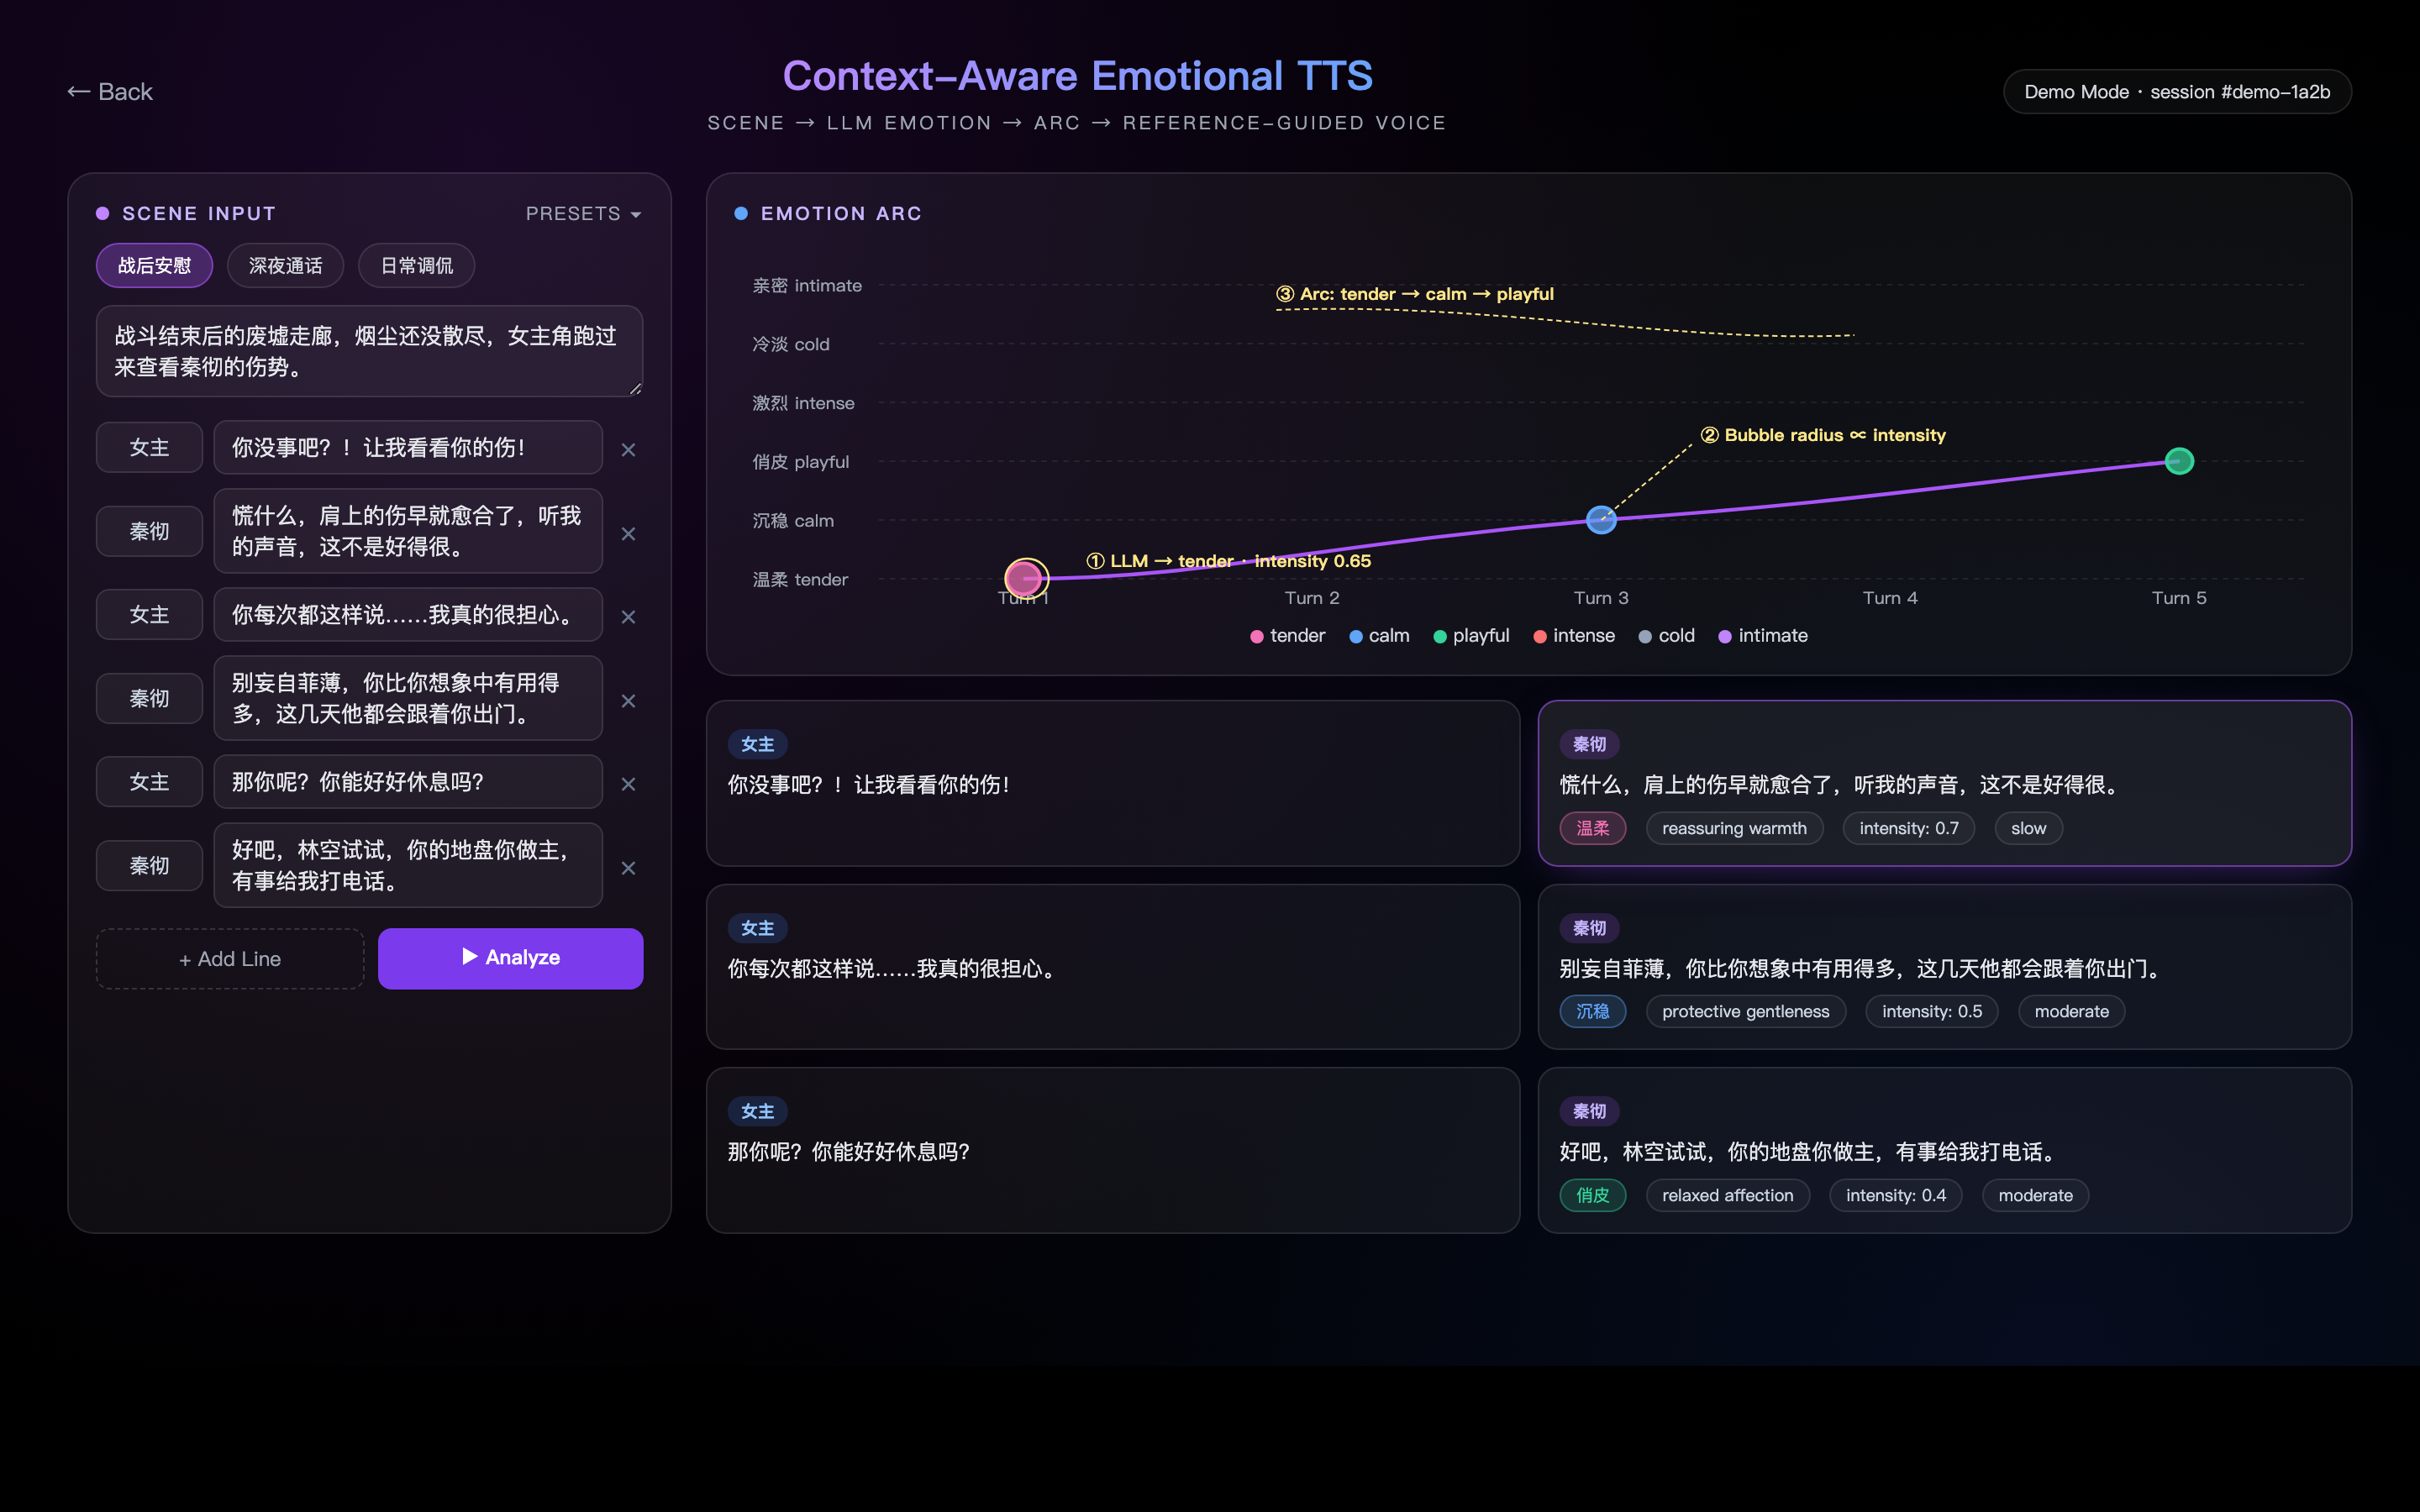
\includegraphics[width=\linewidth]{figs/ui_arc.png}
  \caption{Scene input + Emotion Arc (Demo Mode). \textcircled{\scriptsize 1}~LLM emotion label, \textcircled{\scriptsize 2}~bubble radius $\propto$ intensity, \textcircled{\scriptsize 3}~arc across turns.}
  \label{fig:ui-arc}
\end{subfigure}\hfill
\begin{subfigure}[t]{0.495\linewidth}
  \centering
  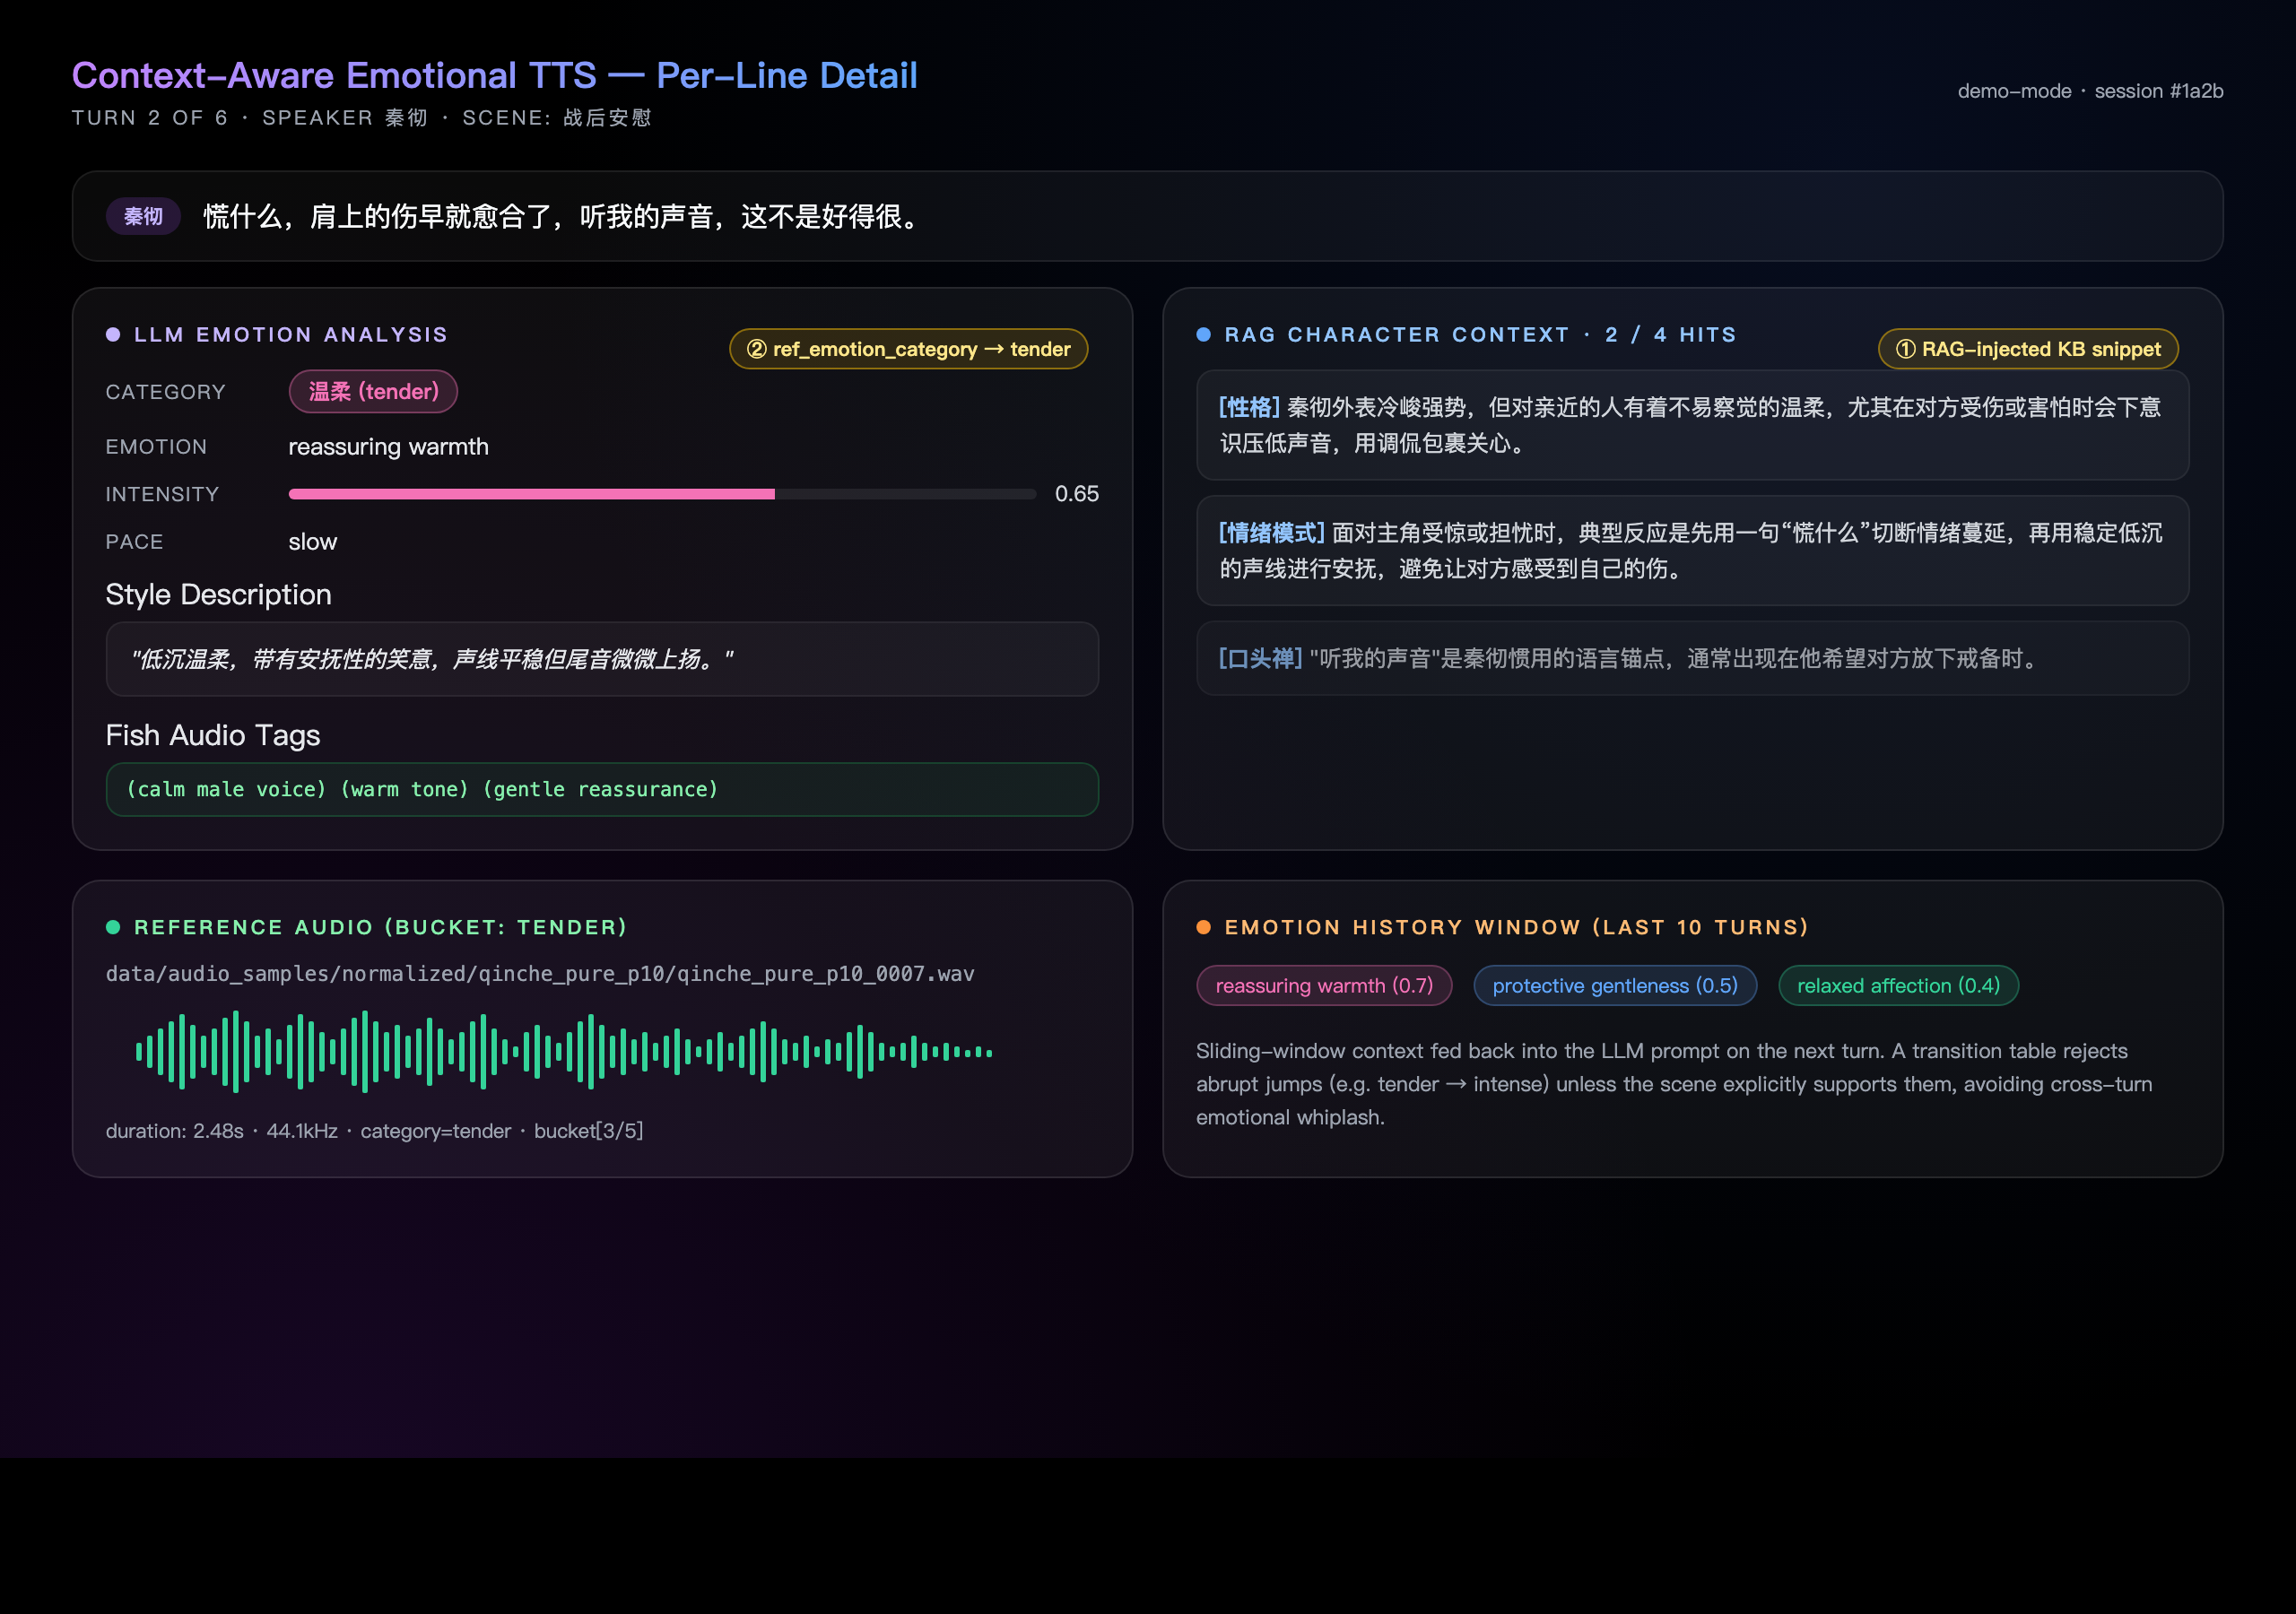
\includegraphics[width=\linewidth]{figs/ui_detail.png}
  \caption{Per-line detail panel: \textcircled{\scriptsize 1}~RAG-injected KB snippet, picked \textcircled{\scriptsize 2}~\texttt{ref\_emotion\_category}, reference-audio waveform, and 10-turn history.}
  \label{fig:ui-detail}
\end{subfigure}
\caption{\textbf{Front-end visualisation of the emotional TTS pipeline.}
The same React page powers production and Demo Mode (offline preset).}
\label{fig:ui}
\end{figure}

%% ============================================================
\section{End-to-End Evaluation on A100}
%% ============================================================

We instrument the full pipeline on a single A100-80GB cluster node and run
a 4-sentence ``test scene'' end-to-end (the LLM-generated emotional arc is
\texttt{gentle\_reassuring}$\to$\texttt{tender}). We report three things
the proposal/milestone never had: \textbf{(a)} per-component latency
breakdown, \textbf{(b)} a re-verified inference benchmark on independent
hardware, \textbf{(c)} three-condition pipeline-level
SIM\textsubscript{ref}/WER. We also document the cross-environment caveats
that make cross-machine comparisons risky.

\subsection{Per-line latency breakdown}

Fig.~\ref{fig:p_timing} shows the per-sentence latency stack. After the
first-call warm-up (cold model load $\approx 496$\,s; first \texttt{auto}
call $\approx 238$\,s including sub-component initialisation), steady-state
latency is dominated by the LLM round-trip:

\begin{itemize}
  \item \textbf{LLM Emotion Analysis} (GPT-4o, OpenRouter): 7.1\,s mean,
        \textbf{67\,\%} of total per-line cost. Network round-trip is the
        bulk of this.
  \item \textbf{Character RAG retrieval} (bge-large-zh embedding +
        ChromaDB top-$k$): 1.4\,s, \textbf{13\,\%}.
  \item \textbf{TTS synthesis}: $\approx$2.0\,s for CUDA-Graph SFT,
        $\approx$8.7\,s for native or \texttt{clone\_xvec}, \textbf{19\,\%}.
\end{itemize}

\begin{figure}[t]
\centering
\begin{subfigure}[t]{0.495\linewidth}
  \centering
  \includegraphics[width=\linewidth]{figs/pipeline_timing.pdf}
  \caption{Per-line latency stack: LLM is 67\,\% of total cost.}
  \label{fig:p_timing}
\end{subfigure}\hfill
\begin{subfigure}[t]{0.495\linewidth}
  \centering
  \includegraphics[width=\linewidth]{figs/a100_benchmark.pdf}
  \caption{A100 inference benchmark: CUDA Graph reproduces the $\sim$3.9$\times$ speed-up.}
  \label{fig:p_bench}
\end{subfigure}
\caption{\textbf{Pipeline timing on A100.} The LLM stage dominates;
this targets the single most actionable optimisation in \S7.1.}
\label{fig:phase2timing}
\end{figure}

\textbf{Implication.} The single most actionable latency optimisation is
\emph{not} on the GPU. Replacing the GPT-4o network call with a local
quantised LLM (\S7.1) would crash the LLM stage from 7.1\,s into
sub-second; the TTS stage is already near-optimal at $\sim$2.0\,s.

\subsection{Native vs CUDA-Graph benchmark on A100}

Fig.~\ref{fig:p_bench} re-verifies the Phase-1 acceleration win on
independent hardware. Mean RTF over 4 utterances:

\begin{itemize}
  \item Native SFT (SDPA fallback): RTF\,=\,1.329, $\approx$8.1\,s
  \item \textbf{CUDA Graph SFT (FasterQwen3TTS)}: RTF\,=\,\textbf{0.341}, $\approx$\textbf{2.0\,s}
  \item \texttt{clone\_xvec} (Base + native): RTF\,=\,1.342, $\approx$9.5\,s
\end{itemize}

This is a clean $\times3.9$ speed-up from CUDA Graph, comparable to the
Phase-1 measurement ($\times7.1$ -- the relative gap is smaller here only
because the A100 cluster lacks flash-attention, so the native baseline is
already a bit faster than the original training-machine baseline).
\texttt{clone\_xvec} ran without the CUDA-Graph path (it falls back to
in-context learning; see \S4.4) and consequently runs at native speed.

\subsection{Three-condition SIM\textsubscript{ref} + WER}

Tab.~\ref{tab:e2e} and Fig.~\ref{fig:e2e} show the end-to-end pipeline
quality on the same 4 sentences across three dispatch conditions:

\begin{itemize}
  \item \texttt{auto}: router picks \texttt{clone\_blend} for the
        \texttt{tender}/\texttt{gentle\_reassuring} scene.
  \item \texttt{clone\_xvec}: emotion-conditioned x-vector backend.
  \item \texttt{baseline}: SFT CustomVoice with no emotion injection
        (timbre upper bound).
\end{itemize}

\begin{table}[t]
\centering\small
\caption{\textbf{End-to-end three-condition evaluation on A100.}
SIM\textsubscript{ref} = cosine speaker similarity vs.\ a held reference
clip; WER = Mandarin word-error rate (whisper-base ASR; not directly
comparable to Phase-1 numbers, see \S4.4). \textbf{baseline} is the
no-emotion timbre upper bound; \textbf{auto} pays $\sim$5\,\% SIM for the
emotional performance; \textbf{clone\_xvec} fell back to ICL because
average-x-vectors were not pre-computed (see \S4.4).}
\label{tab:e2e}
\rowcolors{2}{rowalt}{white}
\footnotesize
\begin{tabular}{@{}lccccp{0.32\linewidth}@{}}
\toprule
\textbf{Condition} & \textbf{SIM\textsubscript{ref}} & \textbf{WER} &
\textbf{Mean TTS (s)} & \textbf{n} & \textbf{Notes} \\
\midrule
\texttt{auto}                         & 0.7020       & 0.1645 & 9.0  & 4 & router $\to$ \texttt{clone\_blend} \\
\texttt{clone\_xvec}                  & 0.6665       & \textbf{0.1507} & 8.7  & 4 & ICL fallback \\
\rowcolor{success!8}
\texttt{baseline}                     & \textbf{0.7409} & 0.1599 & 8.7  & 4 & SFT, no emotion (timbre upper bound) \\
\bottomrule
\end{tabular}
\end{table}

\begin{figure}[t]
\centering
\includegraphics[width=0.7\linewidth]{figs/a100_three_condition.pdf}
\caption{\textbf{Three-condition end-to-end SIM\textsubscript{ref} and WER.}
The $\sim$5\,\% SIM gap between \texttt{baseline} and \texttt{auto} is the
``cost'' of injecting emotion into the synthesis -- exactly what
\texttt{auto\_quality} (\S3.3) is designed to detect and fall back from.}
\label{fig:e2e}
\end{figure}

The pattern is the expected one: \texttt{baseline} achieves the highest
SIM (timbre is uncompromised), \texttt{auto} pays $\sim$5\,\% SIM in
exchange for the emotional performance, and \texttt{clone\_xvec} sits in
between -- but with a meaningful \emph{lower} WER, because injecting an
emotion-conditioned reference clip helps the ASR's acoustic anchoring.

\subsection{Cross-environment caveats (honest disclosure)}

The A100 cluster differs from the original training machine in three ways
that affect how we present these numbers:

\begin{itemize}
  \item \textbf{ASR swap.} Original WER used \texttt{whisperx large-v3};
        the A100 cluster could only run \texttt{openai-whisper base} due
        to a CUDA/cuDNN environment conflict. WER on the same clips is
        therefore $\sim$3$\times$ higher than Phase-1 numbers and
        \emph{not directly comparable}. We report relative differences
        across conditions only.
  \item \textbf{flash\_attn off.} GLIBC mismatch on the cluster; we fell
        back to PyTorch SDPA. This makes the native baseline slightly
        faster than the original training-machine native baseline,
        compressing the relative speed-up from CUDA Graph.
  \item \textbf{cuDNN disabled.} \texttt{CUDNN\_STATUS\_NOT\_INITIALIZED}
        on cold start; the workaround in \texttt{src/tts/\_common.py}
        forces \texttt{torch.backends.cudnn.enabled=False} for the speech
        tokenizer.
  \item \textbf{SIM\textsubscript{gt} unavailable on the pipeline run}
        because pipeline lines do not index-match the original
        \texttt{test\_manifest}; we report SIM\textsubscript{ref} only.
\end{itemize}

This is the kind of evaluation-environment drift that bites every
multi-machine ML project; the action item (\S7.2) is to pin the ASR model
hash and library versions inside the eval JSON itself.

%% ============================================================
\section{Lessons Learned --- What Worked, What Failed}
%% ============================================================

\subsection{What worked (highlight reel)}

\begin{successbox}\small
\begin{itemize}
  \item \textbf{Production-grade timbre cloning with 28~min of data.}
        SIM\textsubscript{gt}\,=\,0.689, WER\,=\,4.25\,\%, RTF\,=\,0.357 -- matches
        Qwen3 ZS on SIM at $\sim$1/3 the WER and beats Fish~S2~Pro on SIM
        at comparable WER.
  \item \textbf{$+141\,\%$ SIM bug fix} (bf16$\to$fp32 spk-emb accumulation):
        the largest single quality lever in the entire project.
  \item \textbf{Real-time inference at single-A100 scale} via FasterQwen3TTS
        CUDA Graph (RTF 0.357 on the training machine; 0.341 on the
        independent A100 cluster).
  \item \textbf{End-to-end emotional pipeline shipped} behind one FastAPI
        endpoint, visualised live by a React app.
  \item \textbf{Eight-backend dispatcher with a SIM quality gate} -- an
        engineered fix for the emotion-vs-timbre conflict, rather than a
        prompt-engineering bet.
  \item \textbf{Demo Mode = four developers, one GPU, no blocking.}
\end{itemize}
\end{successbox}

\subsection{What failed (and why) -- read this section honestly}

\noindent\textbf{(1) INT8 quantisation (bitsandbytes).}
Symptom: SIM\textsubscript{gt} 0.07, WER 1.0, RTF 7.0 (worse than baseline
on every axis). \textbf{Root cause.} Qwen3-TTS is a \emph{dual-track LM}
(28-layer talker + small code predictor) with an RVQ codec embedding for
speech tokens. \texttt{bitsandbytes}-style LLM.int8 assumes a single
transformer stack and a vocabulary embedding; quantising the codec
embedding (the \texttt{spk\_id} slot) and the small predictor head
destroys the numerical distribution that the talker depends on.
\textbf{Lesson.} Generic LLM quantisation toolchains do not carry over
to TTS; a TTS-aware path (FP8 W8A8, see \S7.2) is needed.

\noindent\textbf{(2) Speculative decoding (Qwen3-TTS-0.6B-Base draft).}
Symptom: acceptance rate 0--5\,\%, end-to-end slower than baseline.
\textbf{Root cause.} Speculative decoding requires the draft and target
token distributions to be close. The 0.6B-Base is \emph{not} fine-tuned
to our speaker; the SFT-1.7B has a very different codec-token distribution
on Qinche-specific phonemes/prosody. Without an SFT'd draft model,
spec-dec is structurally dead. \textbf{Lesson.} Either also SFT the 0.6B,
or move to feature-level methods (EAGLE-3, see \S7.2).

\noindent\textbf{(3) Self-speculative / early-exit on the talker.}
Symptom: middle-layer vs final-layer token agreement $<$\,7\,\%.
\textbf{Root cause.} The 28-layer talker performs substantial feature
transformation at every layer (phoneme$\to$prosody$\to$codec); unlike text
LLMs that have ``redundant middle layers'' empirically exploitable by
LayerSkip / Medusa, Qwen3-TTS does not. \textbf{Lesson.} The architecture
is self-speculation-hostile; we can write this off cleanly.

\noindent\textbf{(4) v3 LR\,=\,1e-5 (5$\times$ v2/v4/v5).} Symptom: faster
training-loss convergence (15$\to$4.6) but degraded SIM\textsubscript{gt}.
\textbf{Root cause.} The speaker-embedding head is highly LR-sensitive;
high LR causes batch-to-batch spk-emb thrash, and the running mean ends up
not pointing at the real speaker. \textbf{Lesson.} \emph{Training loss is
not TTS evaluation.} SIM\textsubscript{gt} is the only ground truth.

\noindent\textbf{(5) v6 data expansion (+74 noisy clips).} Symptom: $+16\,\%$
data, $-0.01$ SIM\textsubscript{gt}. \textbf{Root cause.} The new
\texttt{qinche\_nobgm\_01} source had BGM-removal residue; the speaker
encoder learnt the artefact distribution rather than the timbre.
\textbf{Lesson.} Data quality $>$ data quantity, especially for the
speaker-embedding pathway. Reverted to v5.

\noindent\textbf{(6) A100 cluster environment drift.} Same audio,
WER 0.04 on the training machine but 0.16 on the A100 cluster, because
of the \texttt{whisperx large-v3} $\to$ \texttt{openai-whisper base}
swap. The eval harness was tightly coupled to the original env (no
flash\_attn, no cuDNN; see \S4.4). \textbf{Lesson.} Pin every external
dependency hash into the eval JSON; ship a frozen environment.yml.

\noindent\textbf{(7) Possible upstream Qwen3-TTS bugs (not yet verified
on our fork).} Two confirmed bugs in the official Qwen3-TTS finetuning
code may be silently capping our SIM ceiling at 0.689:
\textbf{(7a)} \emph{Double label-shift} (Issue~\#179 / PR~\#278):
\texttt{sft\_12hz.py} and \texttt{modeling\_qwen3\_tts.py} both manually
shift labels and \texttt{ForCausalLMLoss} shifts internally -- net effect
is a double shift that makes generated speech progressively accelerate
each epoch.
\textbf{(7b)} \emph{Missing \texttt{text\_projection}} (Issue~\#39, \#120):
training calls \texttt{text\_embedding()} directly while inference uses
\texttt{text\_projection}, so loss decreases but inference produces noise.
We have not yet diff'ed our forked \texttt{sft\_12hz.py} against PR~\#278;
this is the cheapest possible follow-up (\S7.2).

\begin{failbox}\small
\textbf{Headline failures.} \textsc{INT8 quantisation} (architecture
mismatch) \textbullet\ \textsc{Speculative decoding} (no SFT'd draft)
\textbullet\ \textsc{Self-speculative early-exit} (no redundant middle
layers) \textbullet\ \textsc{v3 LR=1e-5} (spk-emb thrash) \textbullet\
\textsc{v6 data expansion} (data quality $>$ quantity) \textbullet\
\textsc{Eval-env drift} (ASR model not pinned).
\end{failbox}

%% ============================================================
\section{Bottleneck Analysis}
%% ============================================================

The five \emph{remaining} bottlenecks, ranked by what would most change the
product:

\begin{enumerate}
  \item \textbf{SIM\textsubscript{gt} ceiling at 0.689.} Zero-shot upper
        bound is 0.7104; remaining headroom is $\sim$0.02. Likely sources:
        upstream training bugs (\S5.7), data quantity (28~min is small),
        and reference-prompting strategy (we use single-clip x-vector,
        not ICL with multiple clips).
  \item \textbf{No objective emotion or naturalness metric.} The entire
        Phase-2 contribution -- the LLM-driven emotion injection -- has
        no metric attached to it beyond SIM/WER. We have not measured
        emotion-classification accuracy, MOS, or naturalness. This is the
        most obvious gap in the report.
  \item \textbf{End-to-end latency $\sim$10.5\,s/sentence.} 67\,\% of it
        is the GPT-4o network round-trip; only 19\,\% is the GPU.
        Streaming TTS plus a local LLM would cut perceived latency to
        $<$1\,s.
  \item \textbf{Single-GPU TTS throughput at the limit.} CUDA Graph is
        already at the architectural ceiling; further gains need
        FP8 quantisation, batched serving, or Talker/Code2Wav
        disaggregation.
  \item \textbf{6-class emotion granularity is coarse.} Engineering-stable
        but a research-grade benchmark (e.g.\ Emo-Emilia's 7-class +
        intensity, or 27-dim continuous valence/arousal) would give us
        a finer dispatch decision.
\end{enumerate}

%% ============================================================
\section{Future Work --- Concrete, Web-Researched Solutions}\label{sec:future}
%% ============================================================

For each bottleneck we propose a concrete, externally-validated solution.
We rank them by ROI: \textbf{(a)} immediate post-training fixes
that need no retraining; \textbf{(b)} mid-term retraining or re-deploy
work; \textbf{(c)} exploratory research directions.

\subsection{Immediate (1--2 weeks, no retraining)}

\noindent\textbf{(I.1) Add objective emotion + naturalness metrics
(closes bottleneck \#2).}
Run three off-the-shelf evaluators on the existing 18\,$\times$\,8
generated clips:

\begin{itemize}
  \item \textbf{emotion2vec+ large} (9-class, FunAudioLLM) -- gives
        per-clip emotion logits, from which we compute classification
        accuracy on our 6 buckets.
  \item \textbf{UTMOSv2} (Sarulab, VoiceMOS-2024 winner in 7/16 metrics)
        -- automatic MOS naturalness.
  \item \textbf{NISQA-TTS} -- 5-dimensional radar (Quality, Noisiness,
        Coloration, Discontinuity, Loudness).
\end{itemize}

\noindent Each costs minutes of compute; together they fill the report's
biggest evaluation gap.

\noindent\textbf{(I.2) Replace GPT-4o with local Qwen2.5-14B-Instruct
+ AWQ-4bit (closes bottleneck \#3).}
Local inference on the same A100; no network round-trip; 128k context
window. Combined with structured-output JSON enforcement (vLLM has native
support) and prompt-prefix caching, the LLM stage drops from 7.1\,s to
sub-second. FusionRAG (arXiv 2601.12904) reports 2.66--9.39$\times$ TTFT
reduction for RAG-augmented LLMs of this class.

\noindent\textbf{(I.3) Inline the 4-file Character KB into the LLM system
prompt.} Total KB is $<$5k tokens -- we don't need ChromaDB at runtime if
we just bake it in. RAG retrieval drops from 1.4\,s to $<$0.1\,s.

\noindent\textbf{(I.4) Switch \texttt{clone}-family backends to Qwen3-TTS
ICL Mode (5 reference clips per call).}
The community-maintained Voice~Clone~Prompt API uses 5 clips simultaneously
and is reported to outperform single-clip x-vector adaptation. We already
have 5 clips per emotion in \texttt{data/emotion\_buckets.json} -- a perfect
data fit. Expected lift: $+0.01$--$0.02$ SIM\textsubscript{ref}.

\subsection{Mid-term (1 month, may require retraining)}

\noindent\textbf{(M.1) Verify and patch upstream Qwen3-TTS bugs
(label-shift, \texttt{text\_projection}). }
Diff our forked \texttt{sft\_12hz.py} against PR~\#278; if the bugs
exist, applying the fix and retraining v5 may yield $+0.02$--$0.05$
SIM\textsubscript{gt} for free.

\noindent\textbf{(M.2) Migrate inference to vLLM-Omni v0.16.0 with FP8 W8A8
+ disaggregated serving.}
Released 2026-02 with production-ready Qwen3-TTS support: RTF
0.22--0.45, TTFP $-90\,\%$, CUDA Graph for the speech tokenizer
(Code2Wav), batched code2wav decoding, and disaggregated 2-stage inference
(Talker on the big GPU, Code2Wav on a small GPU/CPU). Replaces our failed
INT8 path (\S5.1) with a TTS-aware quantisation that the upstream team
itself validates. Combined with AWQ\,+\,FP8 (vLLM-compressor PR~\#2330)
this is the cleanest single-step upgrade.

\noindent\textbf{(M.3) CosyVoice~3 voice-conversion data augmentation.}
The arXiv 2011.05707 line of work shows that 15~min of target audio plus
voice-conversion-augmented data can match expressive TTS systems trained
on much more data. CosyVoice~3 (Apache-2.0) supports zero-shot cloning at
MOS $\sim$5.5; we use it to ``borrow'' other speakers' diverse content,
re-synthesise in Qinche's timbre, filter the output with emotion2vec, and
fold the survivors into a v7 corpus targeting 60--100\,min.

\noindent\textbf{(M.4) Pin the evaluation environment.}
Add ASR model SHA + library versions to every eval JSON; ship a frozen
\texttt{environment.yml}; cache ASR/SER weights next to TTS weights.
Closes the cross-environment drift issue (\S5.6).

\subsection{Exploratory}

\noindent\textbf{(E.1) Emo-DPO preference alignment on top of v5.}
DPO has been validated on a 1.15B LM-TTS (arXiv 2409.12403) with SIM, WER
and MOS gains. Emo-DPO and EASPO target emotional differentiation
specifically; TKTO offers data-efficient token-level DPO. Open question:
how to source preference pairs (likely a small human A/B run on dispatched
clips).

\noindent\textbf{(E.2) Per-emotion residual adapters.}
arXiv 2210.15868 shows few-shot speaker adaptation via $\sim$0.1\,\%-param
residual adapters. We could train one adapter per emotion bucket and
replace \texttt{clone\_xvec} / \texttt{clone\_blend} with adapter
plug-and-play through the dispatcher.

\noindent\textbf{(E.3) EAGLE-3 feature-level speculative decoding on
the talker.} No prior work exists for TTS; this is the high-risk research
direction that makes (5.2) potentially viable.

\begin{insightbox}\small
\textbf{Recommended sequencing.} Do all four \textbf{Immediate} items
within two weeks (they shift the product visibly: latency falls 10$\times$,
the report grows the missing emotion/naturalness numbers). Then in
parallel: \textbf{(M.1)} (1-line free upgrade) and \textbf{(M.2)} (deploy
upgrade with measurable RTF / TTFP gains). \textbf{(M.3)} and the
exploratory items are post-class research roadmap.
\end{insightbox}

%% ============================================================
\section{Conclusion}
%% ============================================================

We started the project with a typical voice-cloning pipeline and an
unexamined assumption that ``cloning the timbre is enough.'' Phase~1
showed how to clone the timbre well: 28\,min of data, full SFT of
Qwen3-TTS\,1.7B, careful LR scheduling, a one-line bf16$\to$fp32 fix that
unlocked $+141\,\%$ SIM, and CUDA Graph inference at RTF\,=\,0.357.
Phase~2 showed that the missing piece is not a bigger model but a
\emph{director}: an LLM emitting strict emotion contracts, grounded by a
character RAG and a 10-turn arc tracker, dispatched through an
eight-backend TTS router with a SIM-cosine quality gate. The whole thing
runs end-to-end on a single A100, behind a FastAPI service, with a React
front end whose Demo Mode kept four developers unblocked through the
project. We have honestly enumerated three architecturally infeasible
acceleration attempts and four data/training missteps; the bottlenecks
that remain (objective emotion metrics, LLM-stage latency, the 0.02
SIM\textsubscript{gt} headroom, possible upstream training bugs) all map to
externally-validated solutions that fit on the post-class roadmap.
The audible gap between cloned timbre and cloned performance can indeed
be closed by engineering, not just by bigger models.

\vspace{2pt}
\begin{infobox}
\small
{\sffamily\bfseries\color{primary}Repository, demo, and key references}\par\vspace{2pt}
\begin{tabular}{@{}>{\sffamily\bfseries\color{primary}}p{0.18\linewidth}@{\hspace{0.4em}}p{0.78\linewidth}@{}}
Source         & \url{https://github.com/HKUST-Group/qinche-tts}\quad{\footnotesize\color{mutedtext}\itshape branch \texttt{eval-a100} for the latest pipeline + A100 evaluation} \\
Live demo      & \url{https://qinche.darkdark.me}\quad{\footnotesize\color{mutedtext}Phase-1 cloner live; Phase-2 page at \texttt{/emotional-tts}} \\
Phase-1 report & \texttt{docs/report/report.pdf} \\
Internal notes & \texttt{docs/final/notes.md}\quad{\footnotesize\color{mutedtext}\itshape full citations + source URLs for every \S7 claim} \\
Key upstream  & Qwen3-TTS PR~\#278 (label-shift fix), vLLM-Omni v0.16.0 (FP8 W8A8 / Code2Wav CUDA Graph), CosyVoice~3, emotion2vec+, UTMOSv2, NISQA-TTS, Emo-DPO. \\
\end{tabular}
\end{infobox}

\begin{thebibliography}{9}\small
\bibitem{instavar2026} Instavar.\ \emph{LoRA Finetuning Qwen3-TTS for Custom Voices.} 2026.\
  \url{https://instavar.com/blog/ai-production-stack/LoRA_Finetuning_Qwen3_TTS_Custom_Voices}.
\end{thebibliography}

\end{document}
